\chapter{Υλοποίηση}
\InitialCharacter{Σ}το κεφάλαιο αυτό παρουσιάζεται η υλοποίηση της εργασίας. 
Περιγράφεται το περιβάλλον στο οποίο αναπτύχθηκε και
αναλύονται οι γλώσσες και τα εργαλεία προγραμματισμού που επιλέχθηκαν.

\section{Ολοκληρωμένο Περιβάλλον Ανάπτυξης (\en{IDE})}
Η εργασία υλοποιήθηκε στο ολοκληρωμένο περιβάλλον ανάπτυξης \en{IntelliJ IDEA Ultimate 2020}\footnote{\en{https://www.jetbrains.com/idea/}}.
Αυτό είναι ένα λογισμικό ανάπτυξης εφαρμογών που περιλαμβάνει μεταξύ άλλων έναν επεξεργαστή πηγαίου κώδικα,
έναν μεταγλωττιστή και εξειδικευμένα πρόσθετα υποβοήθησης προγραμματισμού. 

Επιλέχθηκε το συγκεκριμένο πρόγραμμα εξαιτίας της καθολικής υποστήριξης των γλωσσών προγραμματισμού που επιλέχθηκαν
και των εργαλείων που χρησιμοποιηθήκαν.

\section{Γλώσσα Προγραμματισμού}
Η γλώσσα προγραμματισμού που επιλέχθηκε για την αναπαράσταση των προδιαγραφών μιας προγραμματιστικής διεπαφής τύπου \en{REST} είναι η \en{Java}.

Η \en{Java} είναι μία γλώσσα αντικειμενοστρεφούς προγραμματισμού 
που σχεδιάστηκε από τον \en{James Gosling} και κυκλοφόρησε από την \en{Sun Microsystems} το 1995.
Οι λόγοι προτίμησης της συγκεκριμένης γλώσσας συμπίπτουν με τους πρωταρχικούς στόχους δημιουργίας της 
και πιο συγκεκριμένα επειδή είναι ανεξάρτητη από την πλατφόρμα του εξυπηρετητή, 
περιλαμβάνει εργαλεία και βιβλιοθήκες διαδικτύου
και έχει σχεδιαστεί για να εκτελεί κώδικα από εξωτερικές πηγές με ασφάλεια \cite{gosling1995java}.

Στο πλαίσιο του αντικειμενοστρεφούς προγραμματισμού,
η \en{Java} χρησιμοποιεί την έννοια της κλάσης
για να προσδιορίζει μια κατηγορία αντικειμένων
και παράλληλα να περιγράφει τα χαρακτηριστικά και τις λειτουργίες τους \cite{arnold2000java}.
Αυτή ακριβώς η έννοια αξιοποιήθηκε για την περιγραφή των προδιαγραφών μιας προγραμματιστικής διεπαφής τύπου \en{REST}
όπως αυτές σχεδιάστηκαν στο Κεφάλαιο 3.

\subsection{Διεπαφές (\en{Interfaces})}
Οι διεπαφές της \en{Java} είναι σύνολα ορισμένων αλλά μη υλοποιημένων λειτουργιών και διαδικασιών.
Αυτές ονομάζονται μέθοδοι και υλοποιούνται από κάποια κλάση\footnote{\en{https://docs.oracle.com/javase/tutorial/java/concepts/interface.html}}.

Αρχικά, δημιουργήθηκαν διεπαφές (\en{interfaces}) για καθένα από τα αντικείμενα που χρησιμοποιηθήκαν,
δηλαδή την προγραμματιστική διεπαφή τύπου \en{REST},
το τελικό σημείο,
τη μέθοδο,
την αίτηση,
την απάντηση,
την κεφαλίδα,
την παράμετρο
και την κατάσταση.
Κάθε διεπαφή περιλαμβάνει τις απαραίτητες διαχειριστικές μεθόδους ανάλογα με τα χαρακτηριστικά της οντότητας που περιγράφει.
Καθεμιά από αυτές ορίζει τη δυνατότητα ενός αντικειμένου να επιστρέφει ως απάντηση στην κλήση της
το αντίστοιχο χαρακτηριστικό των προδιαγραφών. 

Για παράδειγμα, μία διεπαφή προγραμματιστικής διεπαφής περιλαμβάνει μεθόδους για τη διεύθυνση βάσης,
την ετικέτα της
και το σύνολο από τα τελικά σημεία της.

Για λόγους ευκολίας,
από τη στιγμή που η εργασία υποστηρίζει τους τύπους περιεχομένου '\en{application/json}' και '\en{application/x-www-form-urlencoded}',
ο περιορισμός αυτός μεταφέρθηκε στον κώδικα στο σημείο των διεπαφών.
Έτσι, πέρα από την γενική διεπαφή της αίτησης,
υπάρχουν δύο επιπλέον,
η \en{RequestJSON} και η \en{RequestURL} που έχουν προκαθορισμένο τον αντίστοιχο τύπο.
Αυτές είναι που χρησιμοποιούνται στην υπόλοιπη εργασία.

\subsection{Υλοποιήσεις (\en{Implementations})}
Μια κλάση στη \en{Java} θεωρείται ότι υλοποιεί μία διεπαφή όταν
περιλαμβάνει τις μεθόδους που έχουν οριστεί από αυτήν
και περιγράφει τον τρόπο που εκτελούνται από το αντικείμενο.

Επομένως για κάθε διεπαφή δημιουργήθηκε μία αντίστοιχη κλάση,
η οποία υλοποιεί όλες τις μεθόδους και επιπλέον
περιέχει μεταβλητές για τα επιμέρους χαρακτηριστικά της,
καθώς και μία συνάρτηση δόμησης (\en{constructor}). 

Οι κλάσεις ακολουθούν την τεχνική της ενθυλάκωσης (\en{encapsulation}).
Πιο συγκεκριμένα, τα ευαίσθητα δεδομένα των μεταβλητών προστατεύονται από
τις μεθόδους της κλάσης, οι οποίες τα διαχειρίζονται και 
επιτρέπουν την πρόσβαση σε αυτά μόνο για ανάγνωση και όχι για επεξεργασία. 

Όλες οι μεταβλητές των κλάσεων που υλοποιούν διεπαφές είναι ιδιωτικές (\en{private}),
που σημαίνει πως πρόσβαση σε αυτές έχουν μόνο οι μέθοδοι της ίδιας κλάσης.

Αντίθετα, οι διαχειριστικές μέθοδοι που υλοποιούνται είναι όλες δημόσιες (\en{public}).
Αυτό σημαίνει πως ένα αντικείμενο μπορεί να μεταβιβάσει σε οποιοδήποτε άλλο αντικείμενο,
είτε ίδιας είτε διαφορετικής κλάσης,
πληροφορίες για τα χαρακτηριστικά του,
χωρίς όμως να δίνει πρόσβαση στις ίδιες τις μεταβλητές,
κάτι που θα εγκυμονούσε κινδύνους ασφαλείας και προβλήματα αστάθειας.

Για παράδειγμα,
η κλάση που υλοποιεί τη διεπαφή της προγραμματιστικής διεπαφής τύπου \en{REST}
περιλαμβάνει τις ιδιωτικές μεταβλητές της συμβολοσειράς διεύθυνσης βάσης, 
της συμβολοσειράς ετικέτας
και του συνόλου από αντικείμενα της κλάσης του τελικού σημείου.
Για τις τρεις αυτές ιδιωτικές μεταβλητές υπάρχουν οι αντίστοιχες δημόσιες μέθοδοι,
ίδιου τύπου,
χωρίς παραμέτρους,
που έχουν ως έξοδο στην κλήση τους τις αντίστοιχες μεταβλητές.
Τέλος, υπάρχει η δημόσια συνάρτηση δόμησης 
που δέχεται ως παραμέτρους τρεις μεταβλητές,
μία συμβολοσειρά για την διεύθυνση βάσης,
μία συμβολοσειρά για την ετικέτα
και ένα σετ από αντικείμενα τελικού σημείου για τα τελικά σημεία.
Η συνάρτηση αυτή χρησιμοποιείται για τη δημιουργία αντικειμένων της κλάσης της προγραμματιστικής διεπαφής τύπου \en{REST}
με χαρακτηριστικά που αντιστοιχούν στις μεταβλητές που δέχεται ως παραμέτρους.

\subsection{Σχεδιαστικό Πρότυπο}
Ως πρότυπο σχεδίασης της εργασίας επιλέχθηκε αυτό των κατασκευαστών (\en{builder pattern}).
Σκοπός του προτύπου σχεδίασης των κατασκευαστών είναι ο διαχωρισμός της διαδικασίας κατασκευής ενός σύνθετου αντικειμένου από την παρουσίασή του \cite{gamma1995design}.

Με άλλα λόγια,
για κάθε κλάση δημιουργήθηκε μία επιπλέον, 
ένας κατασκευαστής για αντικείμενα της αντίστοιχης κλάσης.
Ο κάθε κατασκευαστής, πέρα από ιδιωτικές μεταβλητές για τα χαρακτηριστικά του αντικειμένου που δημιουργεί,
περιέχει και δημόσιες μεθόδους που επιτρέπουν την επεξεργασία των μεταβλητών.
Αυτές δέχονται μέσω των ορισμάτων τους τιμές για τις αντίστοιχες μεταβλητές
και στο τέλος δημιουργούν ένα αντικείμενο με τα χαρακτηριστικά που έχει δώσει βήμα-βήμα ο προγραμματιστής 
ή το αντικείμενο που καλεί τον κατασκευαστή.

Στη συνάρτηση που δημιουργεί το τελικό αντικείμενο εμπεριέχονται και οι έλεγχοι
για την ορθότητά του με βάση τους περιορισμούς που ορίστηκαν κατά την σχεδίαση των αντικειμένων στο Κεφάλαιο 3.
Εφόσον τα δεδομένα που δέχεται ο κατασκευαστής δεν είναι έγκυρα,
η διαδικασία κατασκευής τερματίζεται και εγείρεται μήνυμα σφάλματος (\en{Runtime Exception}).
Αλλιώς καλείται η συνάρτηση δόμησης της αντίστοιχης κλάσης,
η οποία δέχεται ως ορίσματα τις μεταβλητές του κατασκευαστή με τις τελικές τιμές του,
όπως ορίστηκαν από τις μεθόδους του,
σε μορφή αμετάβλητων (\en{immutable}) αντικειμένων.

Για παράδειγμα, για τη δημιουργία ενός αντικειμένου της κλάσης της προγραμματιστικής διεπαφής τύπου \en{REST},
αρκεί να κληθεί ο αντίστοιχος κατασκευαστής με την εξής μορφή:

\selectlanguage{english}

\begin{lstlisting}[language=java]
    APISpecBuilder newApiBuilder = new APISpecBuilder();
    APISpec newAPI = newApiBuilder
                    .setLabel("api")
                    .setBaseUrl("https://www.example.com/api")
                    .addEndpoint(newEndpoint)
                    .build();
\end{lstlisting}

\selectlanguage{greek}

Με αυτόν τον τρόπο πετυχαίνουμε μεγαλύτερη ευχέρεια στην κατασκευή των αντικειμένων,
ενώ παράλληλα ισχυροποιείται ο έλεγχος που έχει ο προγραμματιστής κατά τη διαδικασία,
ελέγχοντας ταυτόχρονα την εγκυρότητα των δεδομένων.

Οι κατασκευαστές αντικειμένων που έχουν χαρακτηριστικά που αποτυπώνονται με σύνολα,
όπως για παράδειγμα μια προγραμματιστική διεπαφή που μπορεί να έχει πολλαπλά τελικά σημεία,
περιλαμβάνουν μεθόδους για την προσθήκη τόσο ενός από αυτά (πχ. \en{addEndpoint}) 
όσο και περισσοτέρων (πχ. \en{addEndpoints}).
Σε αντίθεση με τις μεθόδους για μεταβλητές που δέχονται μοναδική τιμή και αντικαθιστούν την τιμή με το όρισμα που δέχονται (πχ. \en{setBaseUrl}),
κάθε κλήση μιας μεθόδου προσθήκης δεδομένων διατηρεί τις υπάρχουσες τιμές του συνόλου και προσθέτει σε αυτές τα ορίσματά της.

\section{Κατασκευαστής \en{Groovy}}

Με βάση τη δηλωτική γλώσσα ορισμού μοντέλων διεπαφής που σχεδιάστηκε,
υλοποιήθηκε ένας κατασκευαστής που υποστηρίζει πλήρως τη γραμματική της.
Σκοπός του είναι να δέχεται από τον χρήστη την περιγραφή της διεπαφής για την οποία θέλει να παράξει σενάρια ελέγχου
και να δημιουργεί την αντίστοιχη μοντελοποίηση από αντικείμενα \en{Java}. 
Όπως βλέπουμε και στο σχήμα 4.1, 
στην είσοδό του δέχεται την δηλωτική περιγραφή ενός \en{RESTful API},
την οποία αναλύει με σκοπό να παράξει ένα \en{runtime} μοντέλο του,
δηλαδή στιγμιότυπα (\en{instances}) των κλάσεων \en{Java} που αναπαριστούν τα χαρακτηριστικά του.

Η γλώσσα προγραμματισμού που επιλέχθηκε για την υλοποίηση του συγκεκριμένου κατασκευαστή είναι η \en{Groovy}.
Η \en{Groovy} είναι και αυτή μία γλώσσα αντικειμενοστρεφούς προγραμματισμού,
παρόμοιου συντακτικού με την \en{Java}.
Ένα βασικό χαρακτηριστικό της γλώσσας \en{Groovy} που αξιοποιήθηκε για την εργασία 
είναι η υποστήριξη κομματιών κώδικα που λέγονται \en{closures}.
Ένα \en{closure} μπορεί να ανατεθεί σε μια μεταβλητή,
να δέχεται ορίσματα και να επιστρέφει τιμές.

Στον \en{Groovy} κατασκευαστή που υλοποιήθηκε (\en{Groovy Builder}),
χρησιμοποιήθηκαν ως \en{closures} οι περιγραφές που δίνει ο χρήστης για την προγραμματιστική διεπαφή του και τις ιδιότητές της.
Για παράδειγμα, 
ο ορισμός μιας διεπαφής γίνεται με την κλήση της συνάρτησης \en{api}(),
η οποία δέχεται ως όρισμα ένα \en{closure} στο οποίο περιλαμβάνονται 
η διεύθυνση βάσης, η ετικέτα και τα τελικά σημεία.

Ο τρόπος που θα κατασκευάζαμε μέσω του \en{Groovy Builder} μια προγραμματιστική διεπαφή 
με ένα τελικό σημείο διαπίστευσης χρηστών είναι ο ακόλουθος:

\selectlanguage{english}

\begin{lstlisting}
api {
\end{lstlisting}
\begin{lstlisting}[deletekeywords={api}]
    baseUrl '/test/api'
    label   'my test api'
    endpoint('/login') {
        label 'Endpoint login'
        description 'Endpoint for user login with username and password'
        method('POST') {
            request('URL') {
                withBodyParameter('username', 'String')
                withBodyParameter('password', 'String')
            }
            response('JSON') {
                withStatus(201) {
                    body 'Created'
                }
            }
        }
    }
}
\end{lstlisting}

\selectlanguage{greek}

Επιπλέον ο \en{Groovy Builder} δέχεται υποχρεωτικά ορισμένες πληροφορίες για αρχεία που παράγει η γεννήτρια κώδικα.
Οι πληροφορίες αυτές είναι οι τοποθεσίες, τα πακέτα και τα ονόματα 
του \en{REST API Client} και των σεναρίων ελέγχου,
καθώς και την θύρα (\en{port}) του \en{server} του χρήστη.

\subsection{Μέθοδοι}

\selectlanguage{english}

\begin{lstlisting}
baseUrl(String baseUrl) 
label(String label)
endpoint(String path, Closure configuration)
endpoint(String path, String attribute, Closure configuration)
description(String description)
method(String type, Closure configuration)
request(String type, Closure configuration) # type: JSON or URL
response(String schema, Closure configuration)
withBodyParameter(String name, String type)
withBodyParameter(String name, String type, Object defaultValueIfOptionalAndMissing)
withQueryParameter(String name, String type)
withQueryParameter(String name, String type, Object defaultValueIfOptionalAndMissing)
withHeader(String name)
withHeader(String name, String defaultValueIfOptionalAndMissing)
withStatus(Integer code, Closure configuration)
body(String body)
\end{lstlisting}

\selectlanguage{greek}

\subsection{Μεταβλητές}
\selectlanguage{english}
\begin{lstlisting}
// Rest API Client
clientFolder   # "/Project/src/main/java/"
clientPackage  # "app/restapiclient"
clientName     # "RestAPIClient"
serverPort     # 8765

// Rest API Server Tests
testFolder     # "/Project/src/test/groovy/"
testPackage    # "app/restapitests"
testName       # "TestServer"

// Rest API Client Tests with Mock Server
mockFolder     # "/Project/src/test/groovy/"
mockPackage    # "app/restapimocktests"
mockName       # "MockServer"
\end{lstlisting}
\selectlanguage{greek}


\begin{figure}
    \centering
	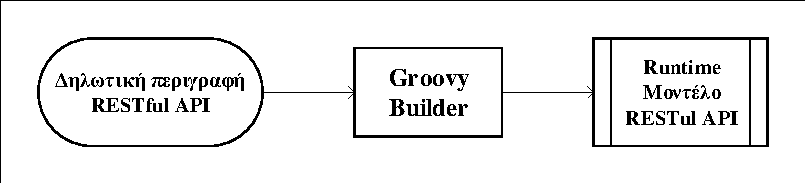
\includegraphics[width=\textwidth]{figures/groovy.pdf}
    \caption{Διάγραμμα ροής κατασκευαστή}
    \label{figure4.1}
\end{figure}

\section{Πλαίσιο Ελέγχου \en{Spock}}
Το \en{Spock} είναι ένα πλαίσιο ελέγχου για \en{Java} και \en{Groovy} εφαρμογές,
ικανό να διαχειριστεί τον πλήρη κύκλο ανάπτυξης ενός λογισμικού
συμβάλλοντας στην αυτοματοποίηση του ελέγχου \cite{kapelonis2016java}.

Με τη χρήση του εργαλείου \en{Spock} πραγματοποιούνται όλοι οι έλεγχοι στο πλαίσιο της εργασίας.
Ο τρόπος με τον οποίο γίνεται αυτό είναι ότι κάθε έλεγχος έχει τη μορφή ενός σεναρίου,
όπου δίνεται μία αρχική κατάσταση 
και παρατηρούμε αν ισχύουν οι συνθήκες που επιθυμούμε μετά την εκτέλεση ορισμένων εντολών. 

Πιο συγκεκριμένα,
για την αξιοποίησή του σε μία εφαρμογή \en{Java} πρέπει 
πρώτα να εισάγουμε την αντίστοιχη βιβλιοθήκη 
και μετά να δημιουργήσουμε κλάσεις \en{Groovy} που επεκτείνουν την '\emph{\en{spock.lang.Specification}}'.
Σε αυτές γράφουμε κομμάτια κώδικα ('\en{blocks}') που ακολουθούν τις φάσεις ('\en{phases}') \en{setup}, 
\en{stimulus}, \en{response} και \en{cleanup}.

Στη φάση \en{setup} ορίζονται οι αρχικές συνθήκες του σεναρίου, 
όπως οι μεταβλητές και τα αντικείμενα που θα χρησιμοποιηθούν στην πορεία.
Στις φάσεις \en{stimulus} και \en{response} περιλαμβάνεται ο κύριος κώδικας του ελέγχου,
όπου εκτελούνται μία ή περισσότερες ενέργειες και ελέγχονται τα αποτελέσματά τους.
Η τελευταία φάση \en{cleanup} αφορά απελευθέρωση πόρων του συστήματος 
και εκτελείται ακόμα κι αν προηγουμένως έχει εγερθεί κάποια εξαίρεση. 

Ο τρόπος με τον οποίο αποφασίζει το \en{Spock} αν ένα σενάριο ελέγχου επιτυγχάνει ή αποτυγχάνει
είναι να παρατηρεί τις συνθήκες που ορίζονται στη φάση \en{response} 
και που αφορούν τα δεδομένα που προκύπτουν από τη φάση \en{stimulus}.
Αν αυτές ικανοποιούνται όλες, 
τότε το σενάριο ελέγχου θεωρείται ότι επιτυγχάνει.
Αλλιώς, αν ακόμα και μία δεν ικανοποιείται, τότε αποτυγχάνει.

Ακολουθεί ένα παράδειγμα χρήσης του εργαλείου \en{Spock}.
Σε αυτό ελέγχουμε αν η διαδικασία αφαίρεσης ενός στοιχείου από μία λίστα ακεραίων αριθμών λειτουργεί σωστά.

\selectlanguage{english}
\begin{lstlisting}
def "Remove element from list"() {
    given:
        def list = [1, 2, 4, 8]

    when:
        list.remove(0)

    then:
        list == [2, 4, 8]
    }
\end{lstlisting}
\selectlanguage{greek}

Στο κομμάτι κώδικα '\en{given}' που αντιστοιχεί στη φάση \en{setup} ορίζουμε την αρχική κατάσταση του σεναρίου ελέγχου 
και πιο συγκεκριμένα δημιουργούμε μία λίστα με τέσσερις ακεραίους αριθμούς.
Στο κομμάτι κώδικα '\en{when}' που αντιστοιχεί στη φάση \en{stimulus} ορίζουμε την εντολή που θέλουμε να εκτελεστεί 
και της οποίας το αποτέλεσμα θέλουμε να ερευνήσουμε. Στην περίπτωσή μας είναι η αφαίρεση του πρώτου στοιχείου από τη λίστα.
Τέλος, στο κομμάτι κώδικα '\en{then}' που αντιστοιχεί στη φάση \en{response} ορίζουμε την συνθήκη που θέλουμε να ισχύει 
μετά το πέρας της εντολής αφαίρεσης, δηλαδή η λίστα να περιέχει πλέον όλα τα υπόλοιπα στοιχεία πέρα από το πρώτο που αφαιρέθηκε.

 
\section{Μηχανή Προτύπων \en{Freemarker}}
Η γεννήτρια κώδικα υλοποιήθηκε με χρήση της μηχανής προτύπων \en{Freemarker}.

Το \en{Freemarker} είναι μία μηχανή προτύπων (\en{Template Engine}) 
που χρησιμοποιείται ως βιβλιοθήκη της \en{Java}
με σκοπό την παραγωγή αρχείων κειμένου,
όπως στην περίπτωσή μας πηγαίος κώδικας.

Για τη λειτουργία της απαιτούνται έτοιμα κομμάτια κώδικα
που προσαρμόζουν τμήματά τους με βάση τα δεδομένα εισόδου της μηχανής προτύπων.
Αυτά τα κομμάτια κώδικα είναι γραμμένη σε μια συγκεκριμένη γλώσσα που ορίζει η βιβλιοθήκη
και τα δεδομένα που προσαρμόζονται λαμβάνονται από αντικείμενα \en{Java}.

Για παράδειγμα,
έστω ότι δίνουμε στη μηχανή προτύπων δώσουμε ένα αντικείμενο διεπαφής με διεύθυνση βάσης '\en{/my/api}'
και το πρότυπο περιλαμβάνει την ακόλουθη γραμμή:

\selectlanguage{english}
\begin{lstlisting}[deletekeywords={api,baseUrl}]
String BASE_URL = "${api.baseUrl}"
\end{lstlisting}
\selectlanguage{greek}

Τότε το παραγόμενο αρχείο θα αντικαταστήσει τη μεταβλητή με την τιμή που δίνει το αντικείμενο:

\selectlanguage{english}
\begin{lstlisting}[deletekeywords={api}]
String BASE_URL = "/my/api"
\end{lstlisting}
\selectlanguage{greek}

\section{Εργαλείο Κατασκευής Λογισμικού \en{Gradle}}
Το \en{Gradle} είναι ένα από τα πιο διαδεδομένα εργαλεία αυτοματοποίησης της κατασκευής λογισμικού.
Υποστηρίζει τις σχετικές διεργασίες όλων των σταδίων ανάπτυξης μιας εφαρμογής, 
από τη μεταγλώττιση του πηγαίου κώδικα μέχρι την εκτέλεση σεναρίων ελέγχου
και τη δημοσίευση του συστατικού (\en{artifact}) σε διαδικτυακές αποθήκες.
Υποστηρίζει πολλές γλώσσες προγραμματισμού,
με τις πιο δημοφιλείς να είναι η \en{Java}, η \en{C/C++} και η \en{JavaScript}.

Το \en{Gradle} λειτουργεί με σενάρια κατασκευής (\en{build scripts})
που περιλαμβάνουν όλα τα \en{projects} που αναλαμβάνει να αναπτύξει.
Κάθε \en{project} αποτελείται από εργασίες (\en{tasks}).
Αυτές είναι εντολές που μπορεί να αφορούν την εκτέλεση κώδικα,
τη μεταγλώττιση ενός προγράμματος και την είσοδο ή έξοδο αρχείων ή καταλόγων.

Για την οργάνωση των εργασιών που πρέπει να γίνουν,
το \en{Gradle} κατασκευάζει έναν κατευθυνόμενο άκυκλο γράφο (\en{DAG})
με βάση τις εξαρτήσεις τους.
Μέσα από τον γράφο καθορίζεται η προτεραιότητα των εργασιών,
καθώς κάθε εργασία για να πραγματοποιηθεί 
πρέπει πρώτα να έχουν ολοκληρωθεί όσες αντιστοιχούν σε προηγούμενους κόμβους.

Η διαδικασία κατασκευής του \en{Gradle} αποτελείται από τρεις φάσεις.
Στη φάση της αρχικοποίησης (\en{Initialization}) ρυθμίζεται το περιβάλλον εργασίας 
και εντοπίζονται τα \en{projects} που παίρνουν μέρος στη διαδικασία.
Στη φάση της διαμόρφωσης (\en{Configuration}) δημιουργείται ο γράφος εργασιων 
και καθορίζεται η σειρά εκτέλεσής τους.
Τέλος, στη φάση εκτέλεσης (\en{Execution}) εκτελούνται οι εργασίες με βάση την προτεραιότητα που αποφασίστηκε πριν.

Για την οργάνωση των \en{projects},
το \en{Gradle} χρησιμοποιεί αρχεία με όνομα '\en{build.gradle}'.
Σε αυτά περιλαμβάνονται όλες οι απαραίτητες πληροφορίες για τις εργασίες του \en{Gradle},
όπως τα \en{plugins} που χρησιμοποιούνται,
τα συστατικά (\en{artifacts}) στα οποία υπάρχουν εξαρτήσεις, καθώς και τα αποθετήρια στα οποία βρίσκονται.
Στο αρχείο αυτό συμπεριλαμβάνονται και οι ορισμοί των εργασιών. 

Στο πλαίσιο της εργασίας,
ο \en{Groovy Builder} υλοποιήθηκε έτσι ώστε να μπορεί να χρησιμοποιηθεί ως ένα \en{Gradle plugin}.
Πιο συγκεκριμένα, 
για τη χρήση του σε ένα \en{project} πρέπει πρώτα να υπάρχει ο αντίστοιχος κώδικας σε έναν φάκελο με όνομα '\en{buildSrc}'.
Στη συνέχεια, 
ο χρήστης με τις παρακάτω εντολές εισάγει τον \en{Groovy Builder} ως \en{plugin}:

\selectlanguage{english}
\begin{lstlisting}[morekeywords={apply,plugin}]
apply plugin: GroovyApiSpecBuilder
\end{lstlisting}
\selectlanguage{greek}

Έπειτα αρκεί να γράψει τον κώδικα στη δηλωτική γλώσσα \en{DSL} που διαβάζει ο \en{Groovy Builder},
καθώς και να παραθέσει τις απαραίτητες πληροφορίες για τον διακομιστή και τους φακέλους αποθήκευσης.
Η παραγωγή των σεναρίων ελέγχου,
καθώς και του κώδικα \en{RESTful API} και των σεναρίων ελέγχου για τον παραγόμενο κώδικα,
πραγματοποιείται με την εντολή '\en{generate}'.